\section{FESDModelv1 Results}
\label{sec:FESDModelv1_results}

Initially, the FESDModelv1 was trained on low-resolution 64x64 pixels images, to improve training and predicting speeds. Further experiments were conducted on higher resolution images. In the next subsections, we present the results of both training variations. Note that the models trained on the low-resolution images were trained for 50 epochs, while when training on images with a higher resolution, the models were trained for 20 epochs due to time limitations.

The results are compared to a baseline model, which solely predicts positive values.

\subsection{Results for low-resolution images}

After training the FESDModelv1 on all four problem sets respectively, we obtained the results, as listed in Table \ref{tab:res_v1}. These are the performance results on the test data, after 50 epochs of training on low-resolution images.

Note that the results of the Joint problem set have been omitted since it suffered from neural collapse. The low resolution of the input images prohibited a reasonable forming of the model.

\begin{table}[!htbp]
  \caption[Test Results of FESDModelv1]{The test results of FESDModelv1 after 50 epochs of training.}
  \label{tab:res_v1}
  \begin{tabular}{lrrrrr}
    \hline
    {} &  Percentage of positive guesses &  Accuracy &  F1-Score &  F2-Score &  Cohen's Kappa Coefficient \\
    Problem Set   &                                 &           &           &           &                            \\
    \hline
    Full Body  &                          50.417 &     0.688 &     0.458 &     0.673 &                      0.397 \\
    Half Body  &                          55.833 &     0.767 &     0.446 &     0.789 &                      0.554 \\
    Body Parts &                          79.028 &     0.779 &     0.722 &     0.842 &                      0.257 \\
    Joints     &                          70.000 &     0.892 &     0.638 &     0.918 &                      0.773 \\
    \hline
  \end{tabular}
\end{table}

FESDModelv1 achieves overall the best F1-Score of $0.77$ on the Half Body problem set. The quality of the model predicting the Half Body problem set is also reflected in the ROC curve as seen in Figure \ref{fig:hb_roc_v1}, with an area under the ROC curve (AUC) value of $0.76$ for the lower body and an AUC of $0.46$.

\begin{figure}[!htbp]
  \centering
  \begin{subfigure}[b]{0.4\linewidth}
      \centering
      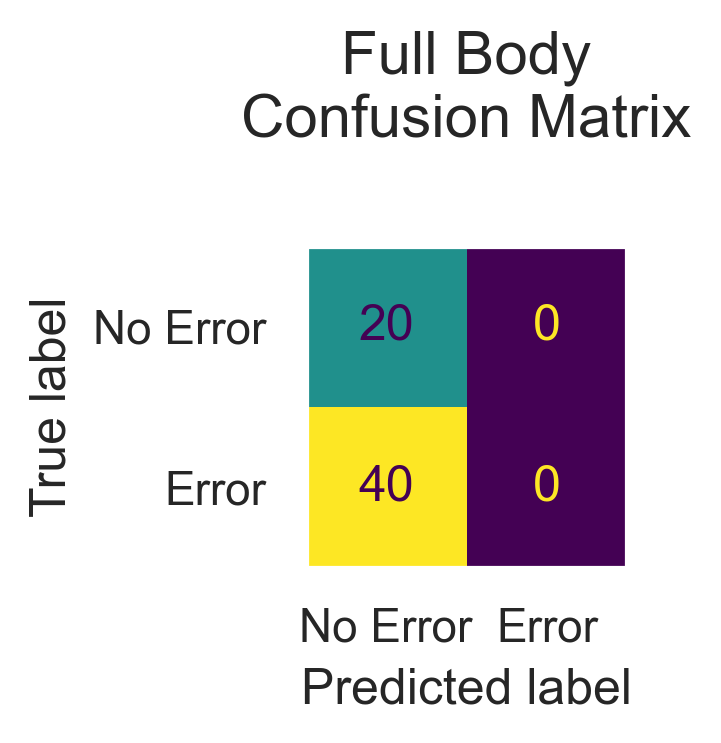
\includegraphics[width=\textwidth]{figures/Results_lo/v1/confusion/full_together.png}
      \caption[]{Full Body Problem Set}
      \label{fig:fb_conf_v1}
  \end{subfigure}
  \hfill
  \begin{subfigure}[b]{0.4\linewidth}
      \centering
      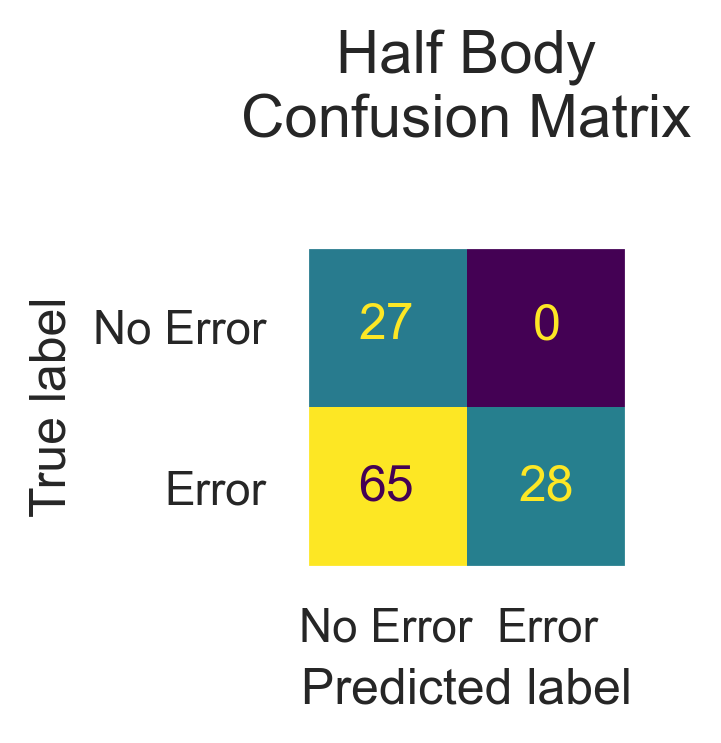
\includegraphics[width=\textwidth]{figures/Results_lo/v1/confusion/half_together.png}
      \caption[]{Half Body Problem Set}
      \label{fig:hb_conf_v1}
  \end{subfigure}
  \hfill
  \begin{subfigure}[b]{0.4\linewidth}
      \centering
      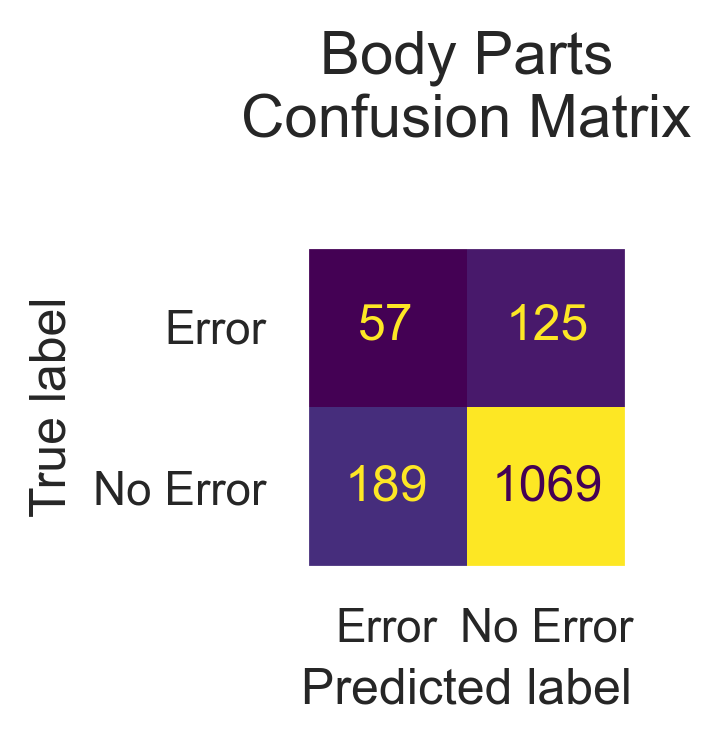
\includegraphics[width=\textwidth]{figures/Results_lo/v1/confusion/body_parts_together.png}
      \caption[]{Body Parts Problem Set}
      \label{fig:bp_conf_v1}
  \end{subfigure}
  \hfill
  \caption[Confusion Matrices of FESDModelv1 (64x64 pixels input resolution)]{The confusion Matrices of FESDModelv1 for the (a) Full Body, (b) Half Body, and (c) Body Parts problem sets trained on input images of 64x64 pixels resolution.}
  \label{fig:conf_v1}
\end{figure}

\FloatBarrier

%
%
%
%
%
%
%
%
%
%
%
%
%
%
%

\subsection{Results for higher-resolution images}

Table \ref{tab:res_v1} shows the results of the testing after 20 epochs of training the models on the Body Parts and Joints problem set on higher-resolution images. The models of each of the two problem sets perform slightly better than the low-resolution images. However, a direct comparison is difficult to make, since the problem sets that are predicted by FESDModelv1 on low resolution images suffer from neural collapse on the higher resolution images and vice versa. When comparing the Body Parts problem set FESDModelv1 performs better, when trained on higher resolution images.

\begin{table}[!htbp]
  \caption[Test Results of FESDModelv1]{The test results of FESDModelv1 after 50 epochs of training.}
  \label{tab:res_v1}
  \begin{tabular}{lrrrrr}
    \hline
    {} &  Percentage of positive guesses &  Accuracy &  F1-Score &  F2-Score &  Cohen's Kappa Coefficient \\
    Problem Set   &                                 &           &           &           &                            \\
    \hline
    Full Body  &                          50.417 &     0.688 &     0.458 &     0.673 &                      0.397 \\
    Half Body  &                          55.833 &     0.767 &     0.446 &     0.789 &                      0.554 \\
    Body Parts &                          79.028 &     0.779 &     0.722 &     0.842 &                      0.257 \\
    Joints     &                          70.000 &     0.892 &     0.638 &     0.918 &                      0.773 \\
    \hline
  \end{tabular}
\end{table}

FESDModelv1 could be trained on the Joint problem set when it is trained with higher resolution input images, resulting in a model that obtains an F1-Score of 0.45. The model might perform better when trained for longer, however, due to time limitations this was not possible and is left for future work.

\begin{figure}[!htbp]
  \centering
  \begin{subfigure}[b]{0.4\linewidth}
      \centering
      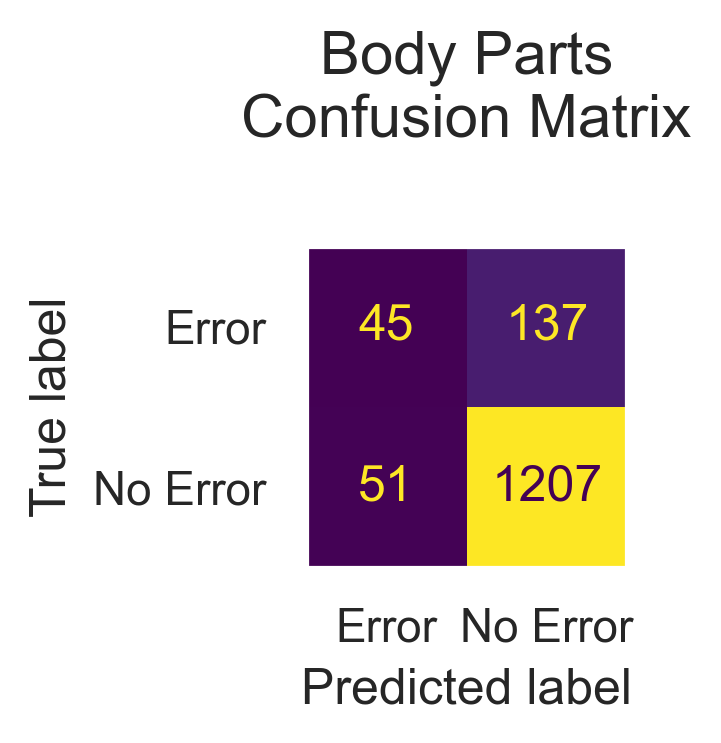
\includegraphics[width=\textwidth]{figures/results_hi/v1/confusion/body_parts_together.png}
      \caption[]{Body Parts Problem Set}
      \label{fig:hi_bp_conf_v1}
  \end{subfigure}
  \hfill
  \begin{subfigure}[b]{0.4\linewidth}
      \centering
      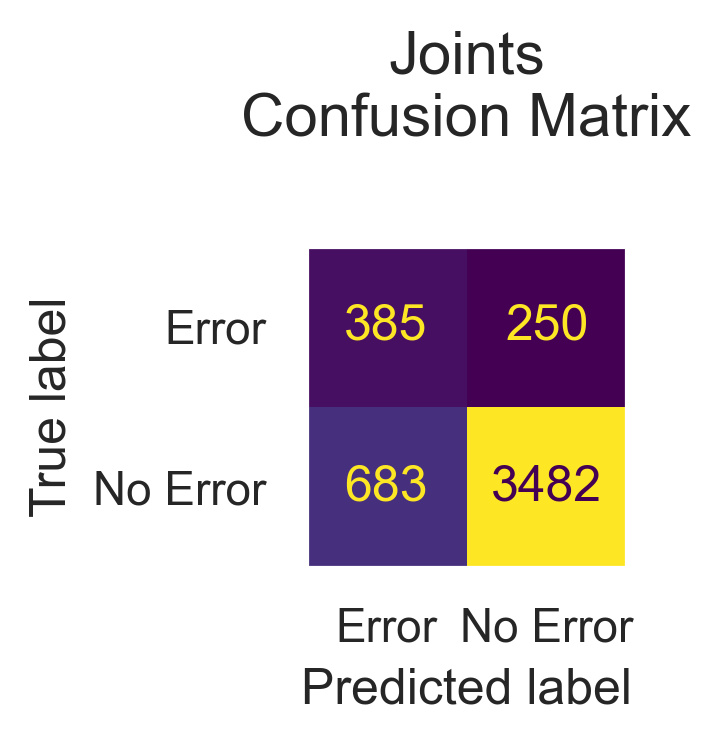
\includegraphics[width=\textwidth]{figures/results_hi/v1/confusion/joints_together.png}
      \caption[]{Joints Problem Set}
      \label{fig:hi_jt_conf_v1}
  \end{subfigure}
  \caption[Confusion Matrices of FESDModelv1 (200x200 pixels input resolution)]{The confusion matrices of FESDModelv1 for the Body Parts, and Joints problem sets.}
  \label{fig:hi_conf_v1}
\end{figure}

\FloatBarrier